\chapter{1-DOF System}
We consider as transfer function from voltage to the mass speed:\\
\\
\[	
G(s)=
\frac{-1.104*10^{5}*s-4.843*10^{-10}}{s^4+41.47*s^{3}+2113*s^{2}+6.275*10^{4}*s-2.268*10^{-9}}
\]
\\
\begin{figure*}[h]
	\centering
	\begin{subfigure}{\columnwidth}
		
	\end{subfigure}
\end{figure*}




\begin{figure}[h]
	\centering
	\subfigure[Bode of G(s)]{Bode_G_1_DOF}
	\quad
	\subfigure[Poles and Zeros of G(s)]{\includegraphics[scale=0.4]{immagini1/PZ_G}}
	\caption{G(s)}
\end{figure}
\\
We have an uncertain resonance frequency, as consequence we cannot delete exactly the resonance peak, but we can only attenuate it, by exploiting the concept of a notch filter related not to a single frequency but to a small bandwidth of 41.3-42.3 rad/s.
\newline 
Applying the notch filter represented in figure \ref{fig:Nf}, we obtain the plant $G_{tot}$(s) of figure \ref{fig:Plant G(s)with Notch Filter1}(b)that is the one we are going to control.
\begin{figure}[h]
	\centering
	\subfigure[Bode diagram]{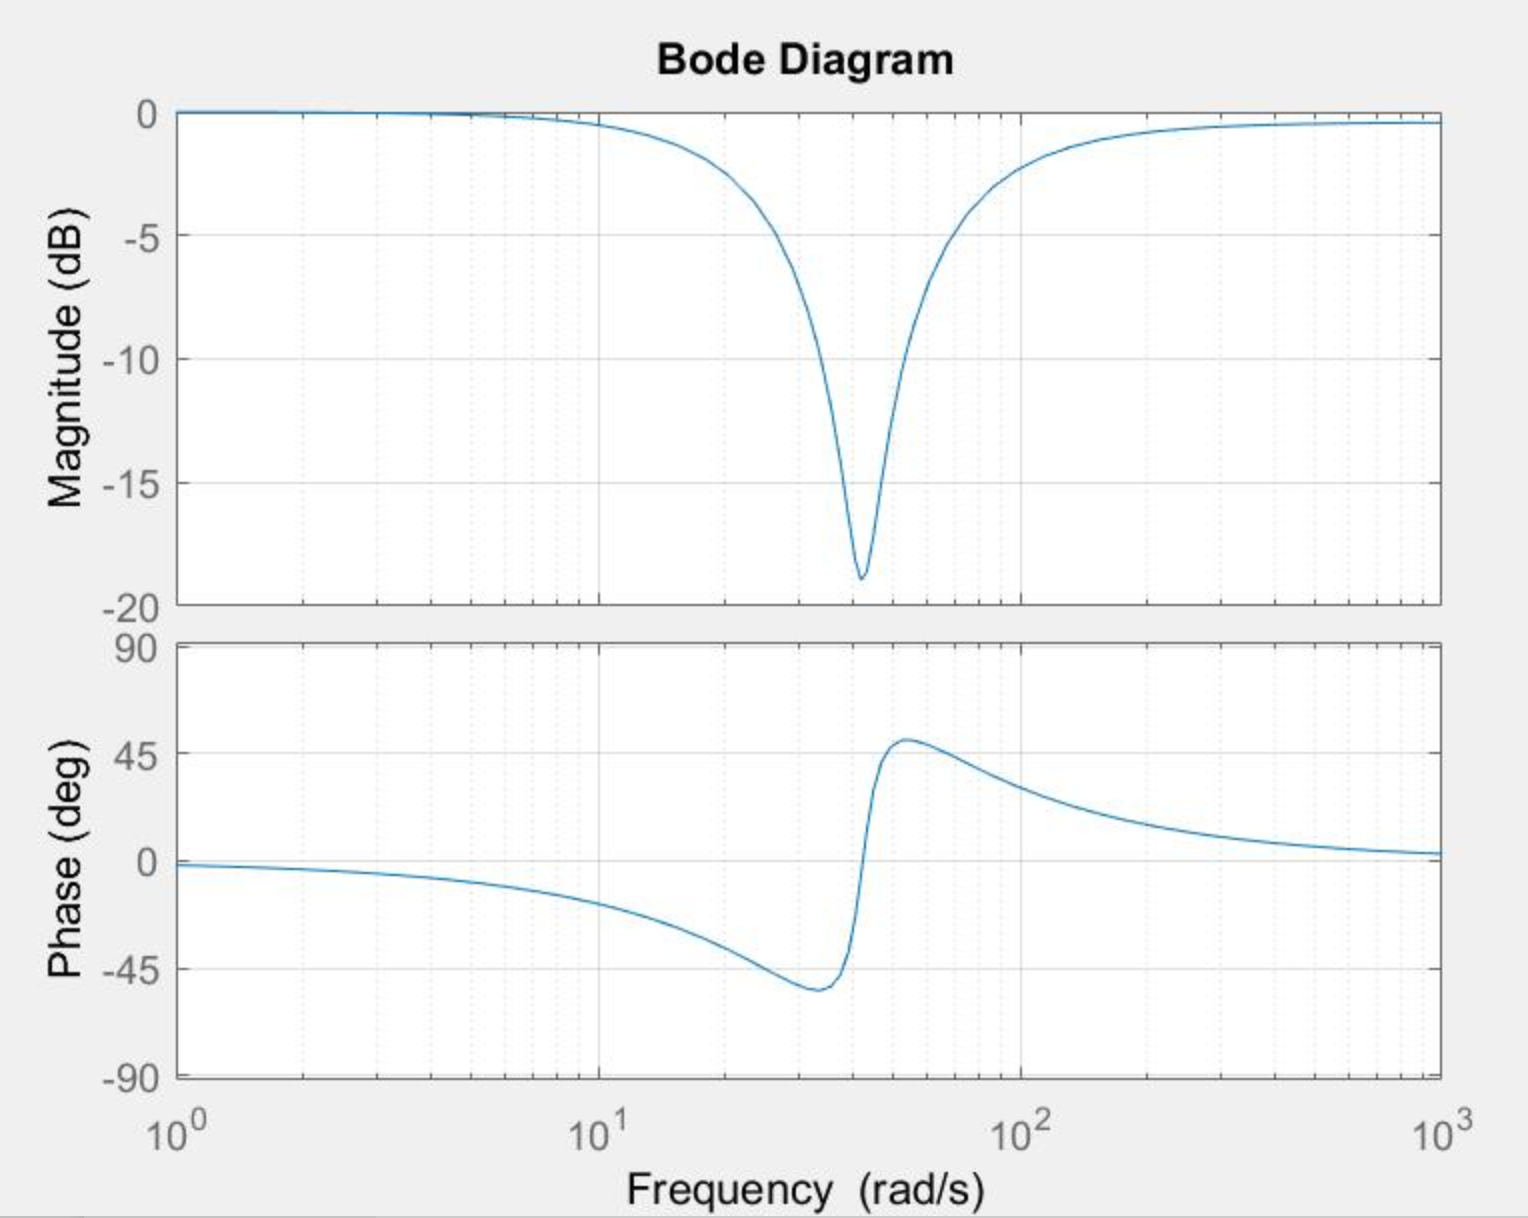
\includegraphics[scale=0.24]{immagini1/Nf}}\quad
	\subfigure[Poles and Zeros]{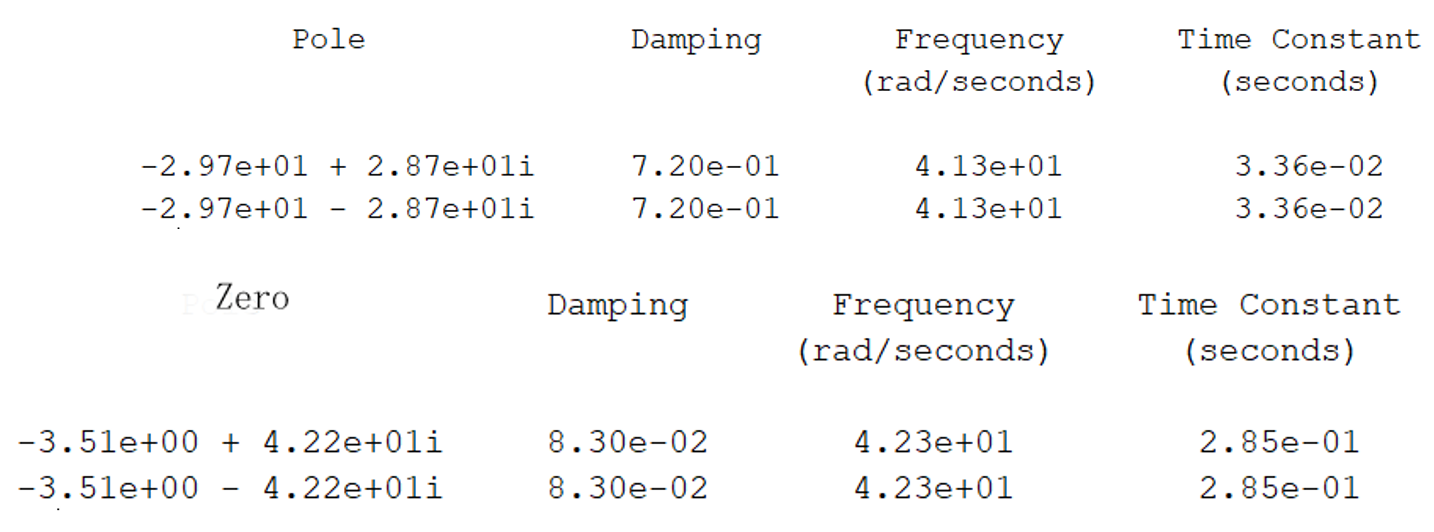
\includegraphics[scale=0.25]{immagini1/PZ_Nf}}
	\caption{Notch filter: Nf(s)}
	\label{fig:Nf}
\end{figure}
\\ \\
\begin{figure}[h]
	\centering
	\subfigure[Bode of G(s) and Nf(s)]
	{\includegraphics[scale=0.5]{immagini1/Nf_G}}\label{fig:Nf1}\quad
	\subfigure[Bode of $G_{tot}$(s)]{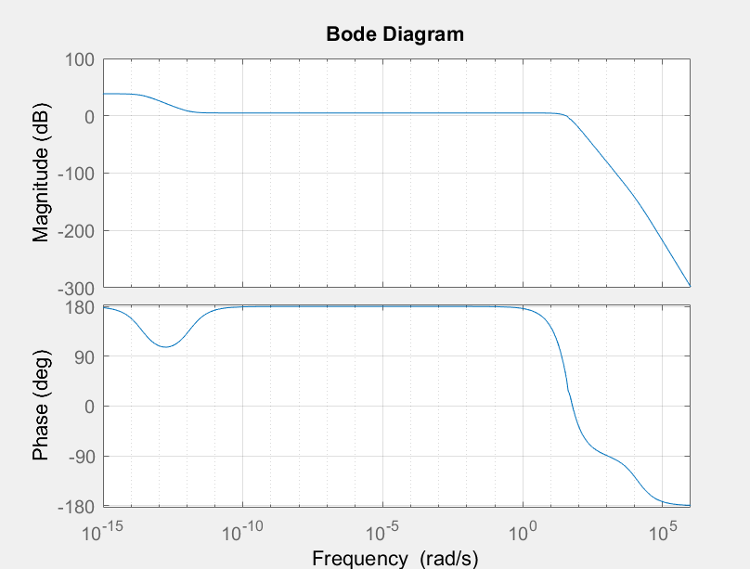
\includegraphics[scale=0.5]{immagini1/Gtot}}
	\label{fig:Gtot}
	\caption{Plant G(s) with Notch Filter: $G_{tot}$(s)}
	\label{fig:Plant G(s)with Notch Filter1}
\end{figure}


\section{Speed Control Loop}
\subsection{Preliminary simulations}
We choose as regulator the PI controller enriched with an anti-windup structure, with which we cancel out the real frequency pole at 33.4 rad/s.
\[
R(s)=-wc_v
\frac{\frac{s}{33.4}+1}{s}
\]
We would like to have a cutting frequency at 10 rad/s,but we notice that, due to the presence of the notch-filter, the cutting frequency imposed by the PI-controller is postponed. 

\begin{figure}[h]
	\centering
	\subfigure[Bode of L(s)]
	{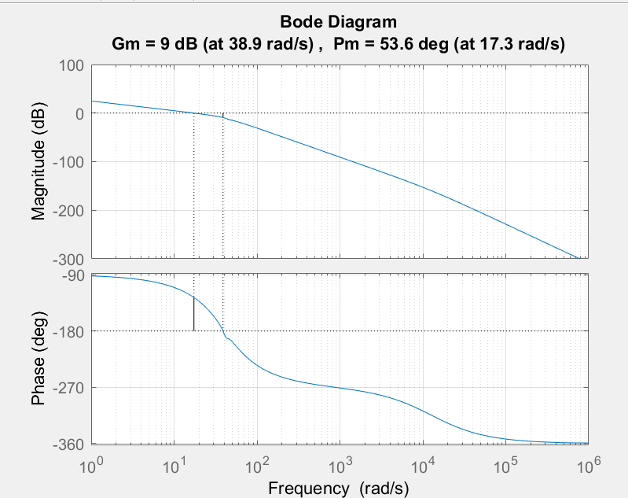
\includegraphics[scale=0.565]{immagini1/Bode_PI_10}}\quad
	\subfigure[Step response]
	{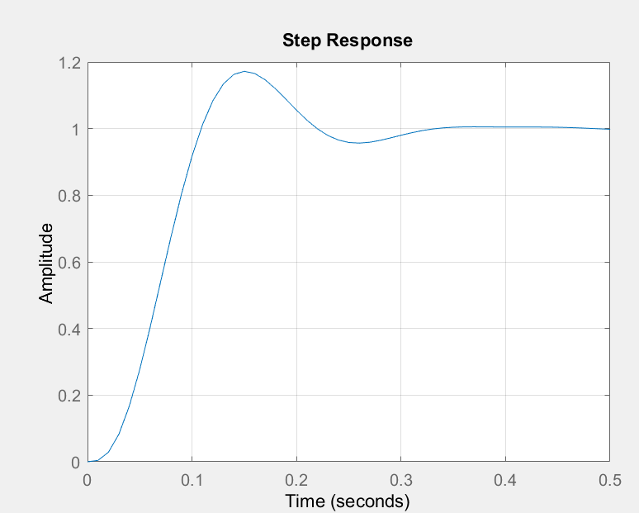
\includegraphics[scale=0.55]{immagini1/Step_PI_10}}
	\label{fig:Step_PI_10}
	\caption{Speed control loop with  $wc_{v} $=10 rad/s}
	\label{fig:Bode and Step PI 10}
\end{figure}


This open loop system would lead us to the step response of the figure \ref{fig:Bode and Step PI 10}(b). 
Even if this response could be considered acceptable, we have to remember that this is just a simulation. Having such a low phase margin could generate undesidered behavior in presence of disturbance of the real system.

\par
In order to have a more robust control system, it is so necessary to increase the phase margin by reducing the cutting frequency. We simulate for this reason a unitary step response with different bandwidth of the speed loop in figure \ref{fig:Step with many wc} and then we will choose the ones we like the most.
\begin{figure}[h]
	\centering
	\includegraphics[scale=0.7]{immagini1/Step_PI_many}
	\caption{Step response with several $wc_{v} $}
	\label{fig:Step with many wc}
\end{figure}
\newline We have focused on three possible values of $wc_{v} $: 5.5 , 6 , 7 rad/s.
So we plot the corresponding simulink schemes in order to better evaluate the system behaviour; in particular we have considered one of the worst case scenarios, that is the step from -17 rad/s to 17 rad/s, and then we apply a step of 10 rad/s. The first one lets us to asses the voltage saturation while the second one the transient after an ordinary step.
\begin{figure}[h]
	\centering
	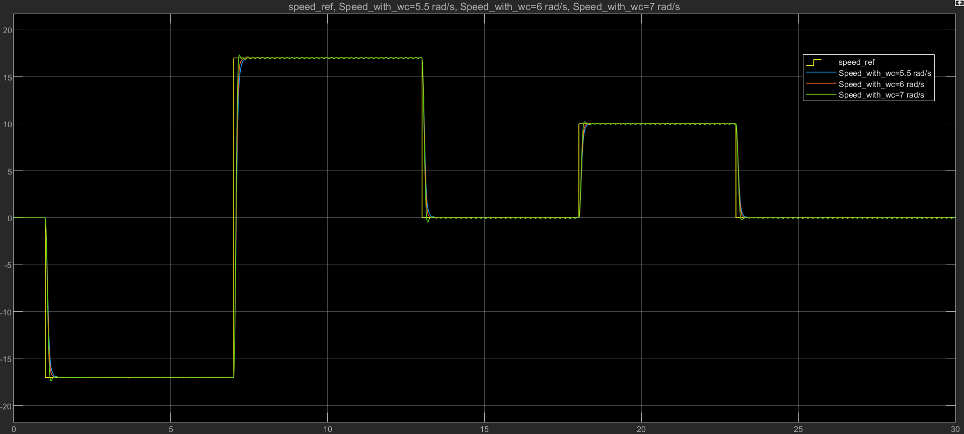
\includegraphics[scale=0.45]{immagini1/Sim_PI_567}
	\caption{Step response with the three different $wc_{v} $}
\end{figure}
\par For the reason that the notch filter slows down the control action that comes out from the PI with anti-windup, we would like to avoid a control system in which the signal after the notch filter, which is the voltage, saturates. We plot now the voltage of the three different cases so that we can choose for the fastest controller that satifies this requirement: 
\begin{itemize}
	\item $wc_{v} $= 5.5 rad/s
	\begin{figure}[h]
		\centering
		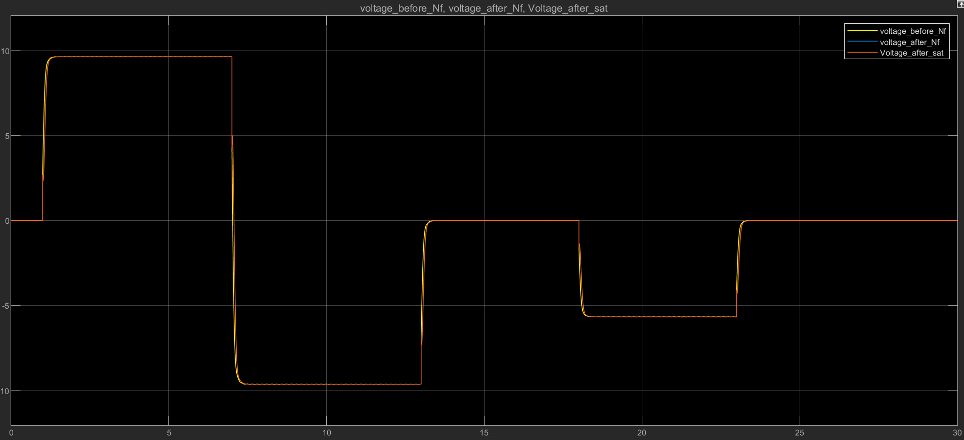
\includegraphics[scale=0.42]{immagini1/Volt_PI_5}
		\caption{Voltage with $wc_{v} $=5.5 rad/s}
	\end{figure}
	
	\item $wc_{v} $= 6 rad/s 
	\begin{figure}[h]
		\centering
		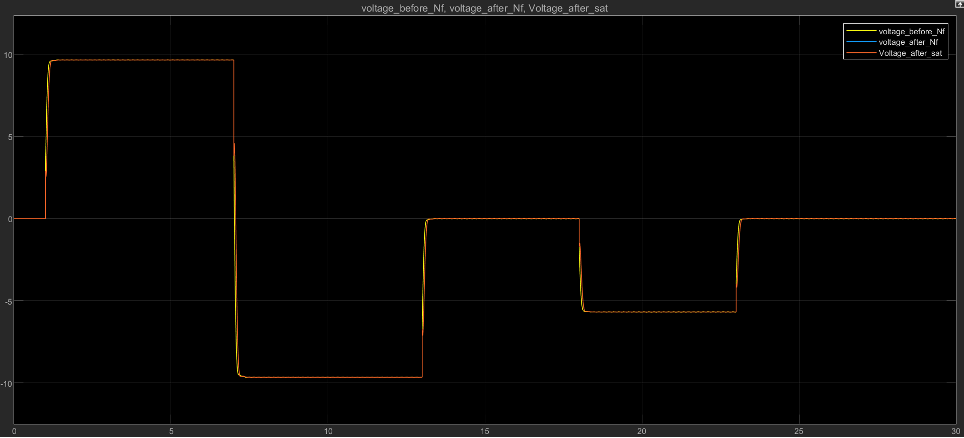
\includegraphics[scale=0.42]{immagini1/Volt_PI_6}
		\caption{Voltage with $wc_{v} $=6 rad/s}
	\end{figure}
	\item $wc_{v} $= 7 rad/s
	\\
	\begin{figure}[h]
		\centering
		\subfigure[Voltage plot]
		{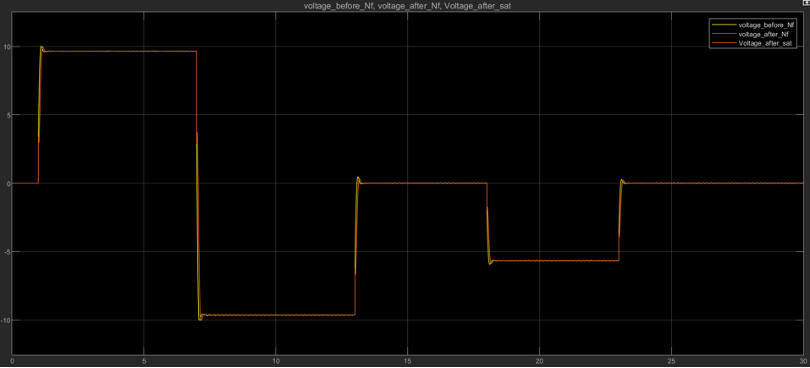
\includegraphics[scale=0.42]{immagini1/Volt_PI_7a}}\quad
		\subfigure[Saturation detail]
		{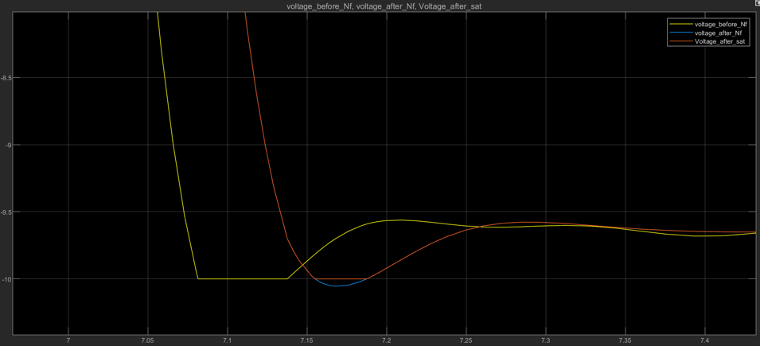
\includegraphics[scale=0.45]{immagini1/Volt_PI_7b}}	
		\caption{Voltage with $wc_{v} $=7 rad/s}
	\end{figure}
\end{itemize}

\par
Analysing the above plots, we can notice that for $wc_{v} $ equal to 5.5 and 6 rad/s voltage never saturates, whereas for $wc_{v} $ = 7 rad/s it does. As a result, we choose $wc_{v} $=6 rad/s. 
By doing this, we ensure a cutting frequency of 14 rad/s and a phase margin of 61 deg, improving even our initial target!
The bode plot of the final speed open loop is represented in the figure \ref{fig:Bode_L_PI}.
\begin{figure}[h]
	\centering
	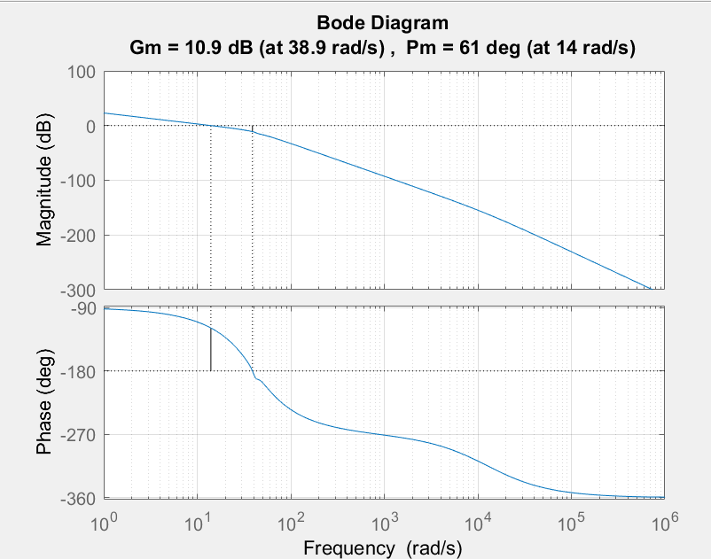
\includegraphics[scale=0.45]{immagini1/Bode_L_PI}
	\caption{Bode of L(s)}
	\label{fig:Bode_L_PI}
\end{figure}
\subsection{Laboratory experiments}
Starting from what we have said before, in the laboratory we make different tests. In general, we notice that if we apply to the real system the same controller parameters, we have chosen previously, we obtain a more aggressive response that cannot be accepted. This concept can be shown in this plot, in which we evaluate the system response with three different $wc_{v} $= [3.5,4,5] rad/s. 
\begin{figure}[h]
	\centering
	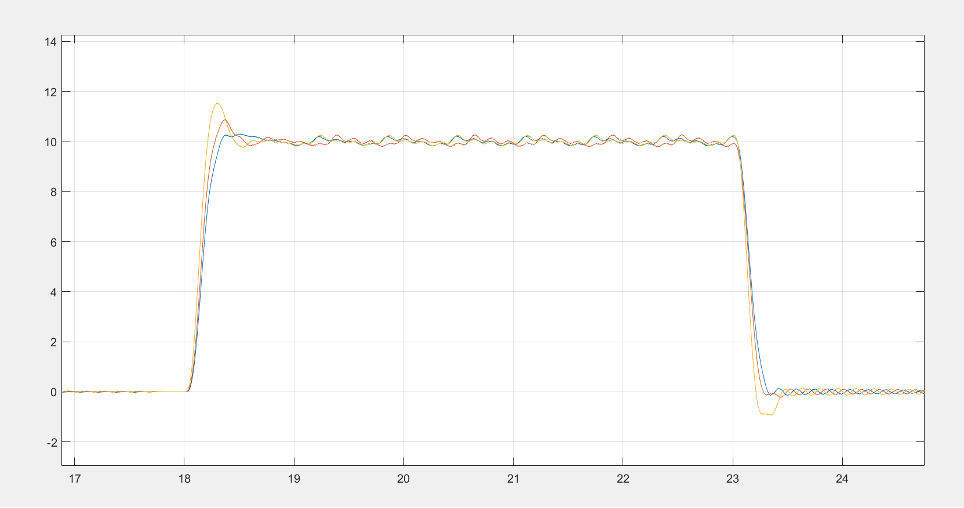
\includegraphics[scale=0.5]{immagini1/LAB_PI}
	\caption{Step response for $wc_{v} $=3.5 rad/s, $wc_{v} $=4 rad/s, $wc_{v} $=5 rad/s }
	\label{fig:LAB_PI}
\end{figure}
As can we notice in our simulations at home, putting $wc_{v} $= 5 rad/s led to a very smooth response, while in the laboratory, the same controller can be considered even too aggressive, as it is possible to see in the plot in figure \ref{fig:LAB_PI}. We choose so for the solution made with $wc_{v} $=3.5 rad/s.
\newline
We observe the presence of very small oscillations, their frequencies are equal to the speed, so we suppose that it depends on a change of the dynamic friction coefficient value along the revolution. As a matter of fact, this undesired behaviour can be neglected, since the amplitude of the above-mentioned oscillations is very small.   In the case in which we would like to attenuate them, we should increase the bandwidth of the loop to counteract them on time. By using just a PI this is not possible, because if we increase $wc_{v} $, we face significant oscillations, that cannot be accepted. To avoid this behavior, we could just put a low pass prefilter on the reference signal, in this way a possible step on the speed reference would be made smoother and just small oscillations should arise. This solution will be analized with more details in the 2-DOF case, in which these oscillations at the steady state cannot be neglected.
\section{Position Control Loop}
\subsection{Preliminary simulations}
To control the position, we decide to use a cascade strategy: the inner loop controls the speed, whereas the outer one the position.
For the first loop we use the same PI structure as explained above, while the position is regulated by using a proportional controller.
It is important to remark that the cutting frequency of the position and the speed one must be far enough (about one decade) to assure the frequency decoupling of the two loops. As consequence if we maintain the cutting frequency of the speed loop as decided before ($wc_{v} $=6 rad/s that corresponds to a bandwidth of 14 rad/s), a first possible solution is reached by setting the position cutting frequency equal to 1.4 rad/s. This case is represented in the figure \ref{fig:System with 1.4}. From these plots we can see the overall system is very robust but also very slow.
\\

\begin{figure}[h]
\centering
\subfigure[Bode diagram]
{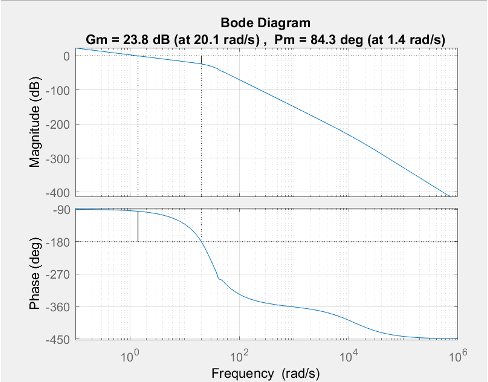
\includegraphics[scale=0.72]{immagini1/Bode_P_1.4}}\quad
\subfigure[Step response]
{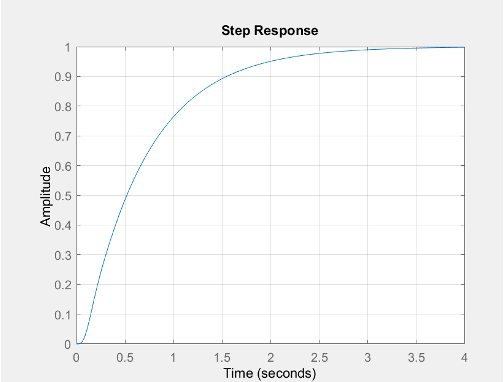
\includegraphics[scale=0.72]{immagini1/Step_P_1.4}} 
\caption{System with $wc_{p} $=1.4 rad/s}
\label{fig:System with 1.4}
\end{figure}

\begin{figure}[h]
	\centering
	\subfigure[Bode diagram]
	{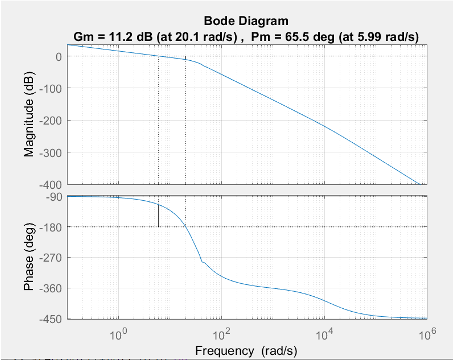
\includegraphics[scale=0.81]{immagini1/Bode_P_6}}\quad
	\subfigure[Step response]
	{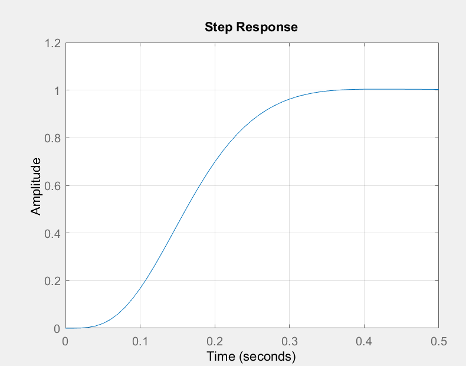
\includegraphics[scale=0.8]{immagini1/Step_P_6}} 
	\caption{System with $wc_{p} $=6 rad/s}
	\label{fig:System with 6}
\end{figure}

On the other hand, we can accept even a ratio between the speed cutting frequency and the position one up to 50 \%. In this scenario we can fix the proportional gain around 6 rad/s, and we can notice (figure \ref{fig:System with 6}) that the position loop is not so influenced by the inner one. 

\par 
We consider now the Simulink simulation with $wc_{p} $=6 rad/s (figure \ref{fig:Ref_Track_P_6}), because, thanks to the saturation, it better represents the real dynamics and we are so able to evaluate overshoots and the control effort.
\begin{figure}[h]
	\centering
	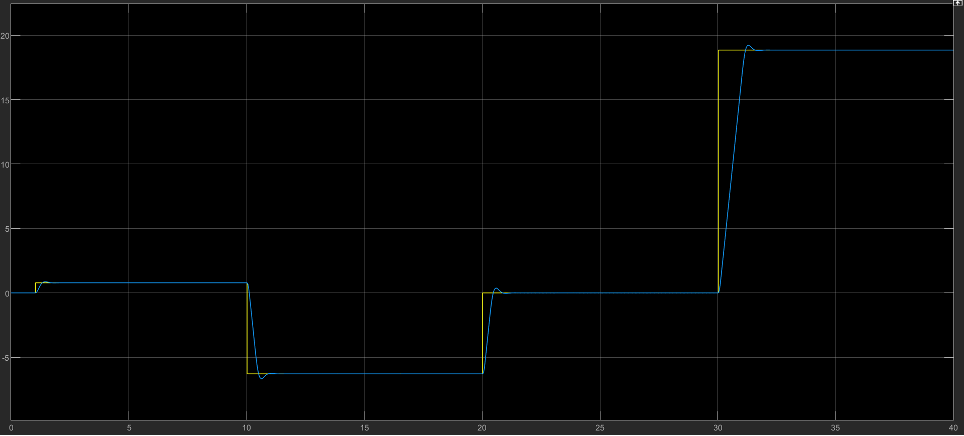
\includegraphics[scale=0.75]{immagini1/Ref_Track_P_6}
	\caption{Reference tracking with $wc_{p} $=6 rad/s }
	\label{fig:Ref_Track_P_6}
\end{figure}
By the way, the solution plotted in the figure \ref{fig:Ref_Track_P_6} has significant overshoots, that is a behavior which we would like to avoid in the position reference tracking, at least during the simulation part. For this reason, we provide two other solutions that still let us have an acceptable settling time:
\begin{itemize}
	\item High-pass pre-filter  and $wc_{p} $=1.4 rad/s:
	\newline
	Applying a pre-filter at the reference position, we are able to increase the position reference value for a small amount of time. This let us have even a smaller transient time than the previous one.
	In this case we impose the position cutting frequency at 1.4 rad/s. In this way we easily decouple the dynamics of the inner and outer loop. 
	\[
	\centering
	Pf(s)=
	\frac{\frac{s}{1.4}+1}{\frac{s}{5}+1}
	\]
	\begin{figure}[h]
		\centering
		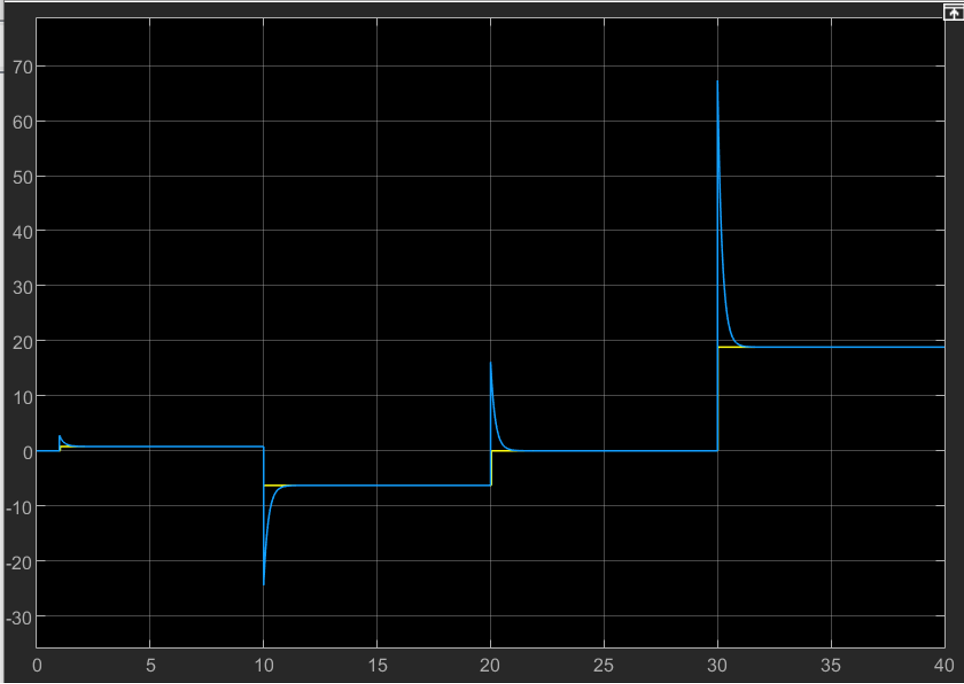
\includegraphics[scale=0.37]{immagini1/Pf_1.4}
		\caption{Position reference signal prefiltered and not }
	\end{figure}
\item 	$wc_{p} $=3.6 rad/s:
\newline This solution, that does not contemplate the presence of the high pass prefilter, is made by setting the outer cutting frequency equal to 3.6 rad/s, finding so a trade off between the two banwidths compared above.	
\end{itemize}

\par 
We plot now the reference tracking and the control effort of the three possible solutions we have explained, in order to choose the one we like the most. While the plot in figure \ref{fig:Pos_ref_comparison} shows the whole time domain of the simulation, the voltage plots in figure  \ref{fig:Volt_sat_comparison} only show the first 12 seconds. We did in this way otherwise the analysis of the saturation would have been impossible. After this analysis we choose for $wc_{p} $=3.6 rad/s.

\begin{figure}[h]
	\centering
	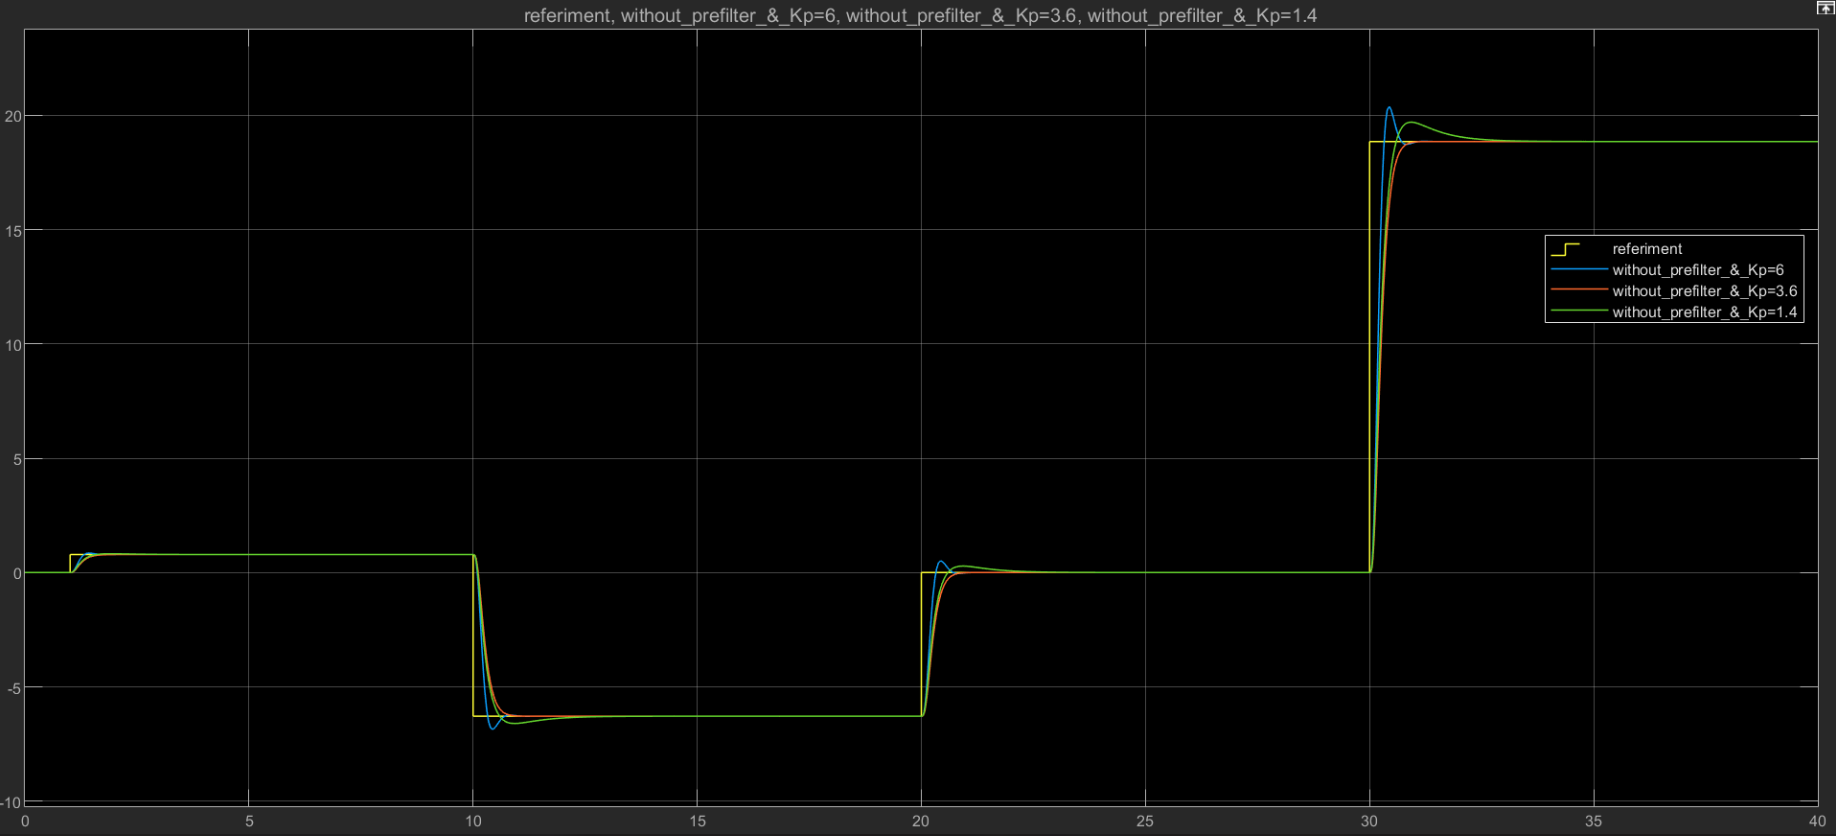
\includegraphics[scale=0.38]{immagini1/Sim_many_P}
	\caption{Comparison of the position reference tracking}
	\label{fig:Pos_ref_comparison}
\end{figure}
\begin{figure}[h]
	\centering
	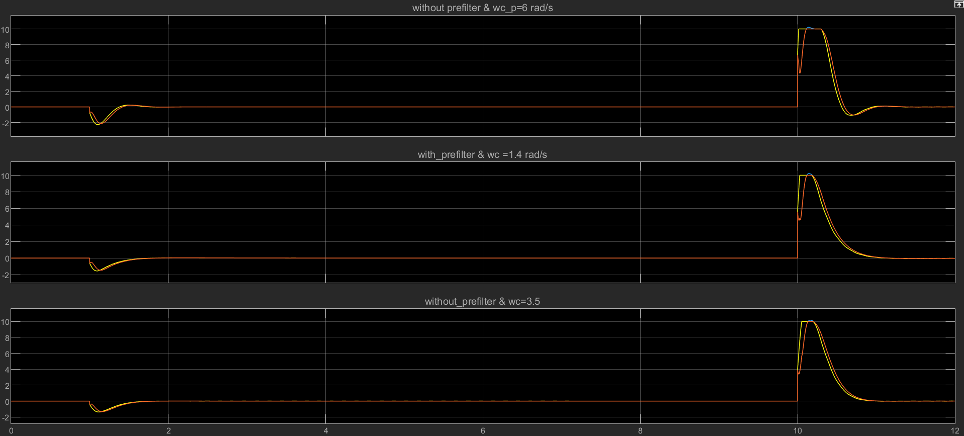
\includegraphics[scale=0.75]{immagini1/Volt_sat_P}
	\caption{Comparison of the control efforts of the first 12 seconds}
	\label{fig:Volt_sat_comparison}
\end{figure}

\subsection{Laboratory experiments}
After some tests done in the laboratory, we compare the three most significant solutions. For all three of them, the inner loop is the same and it coincides with a PI regulator with anti-windup set with $wc_{v}$=5 rad/s (as analized in the section 1.1.2). However, we should remember that, for the reason explained in the speed control loop section, $wc_{v}$ is only a parameter and it does not represent the real banwidth of the inner loop, which we reckon to be around 15 rad/s.
During the tuning of the speed controller, we considered the open loop made through $wc_{v}$=5 rad/s too much aggressive; yet, considering the cascade control strategy, the inner loop never receives a step as reference signal, we are so allowed to speed up the inner controller so as to enlarge the bandwidth of the outer loop and satisfy the frequency decoupling at the same time.
The three solutions differ with respect to the proportional gain $k_{p}$:
\begin{itemize}
	\item $k_{p}$=2 rad/s;
	\item $k_{p}$=6 rad/s;
	\item $k_{p}$= 4 rad/s and a pre-filter of $P_{f}$(s)=$\frac{\frac{s}{4}+1}{\frac{s}{6}+1}$;
\end{itemize}

\begin{figure}[h]
	\centering
	\subfigure[Position reference tracking]
	{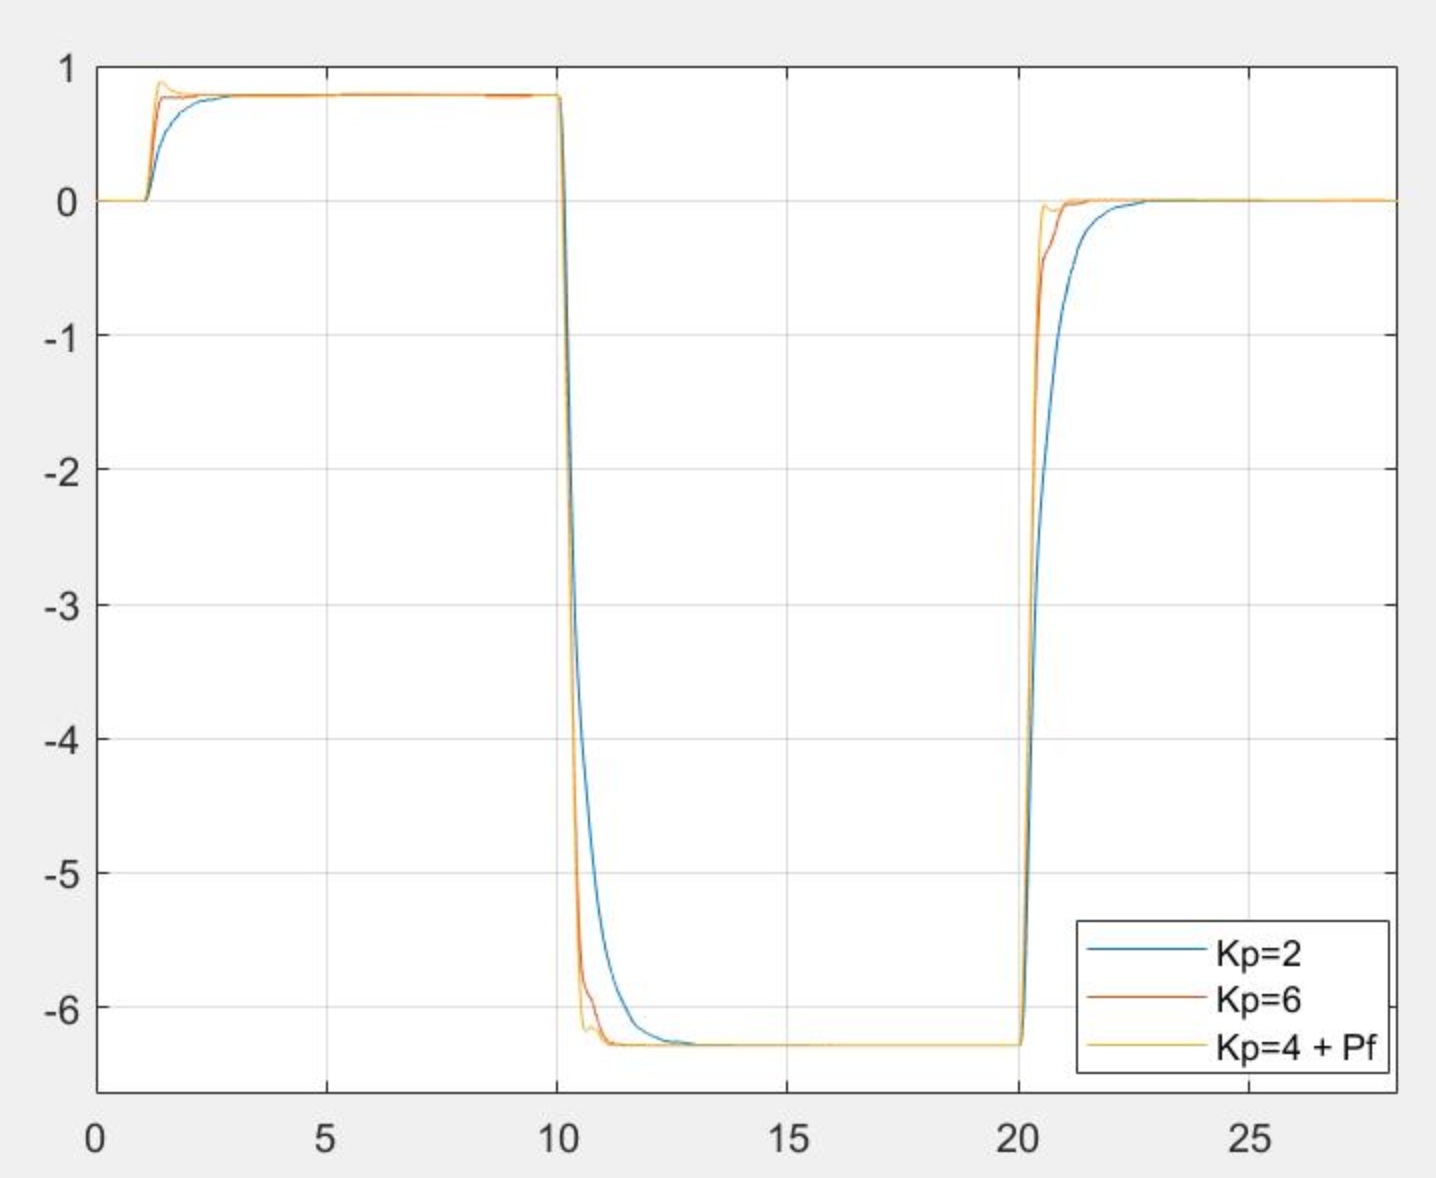
\includegraphics[scale=0.255]{immagini1/LAB_P_pos}} \quad
	\subfigure[Voltage]
	{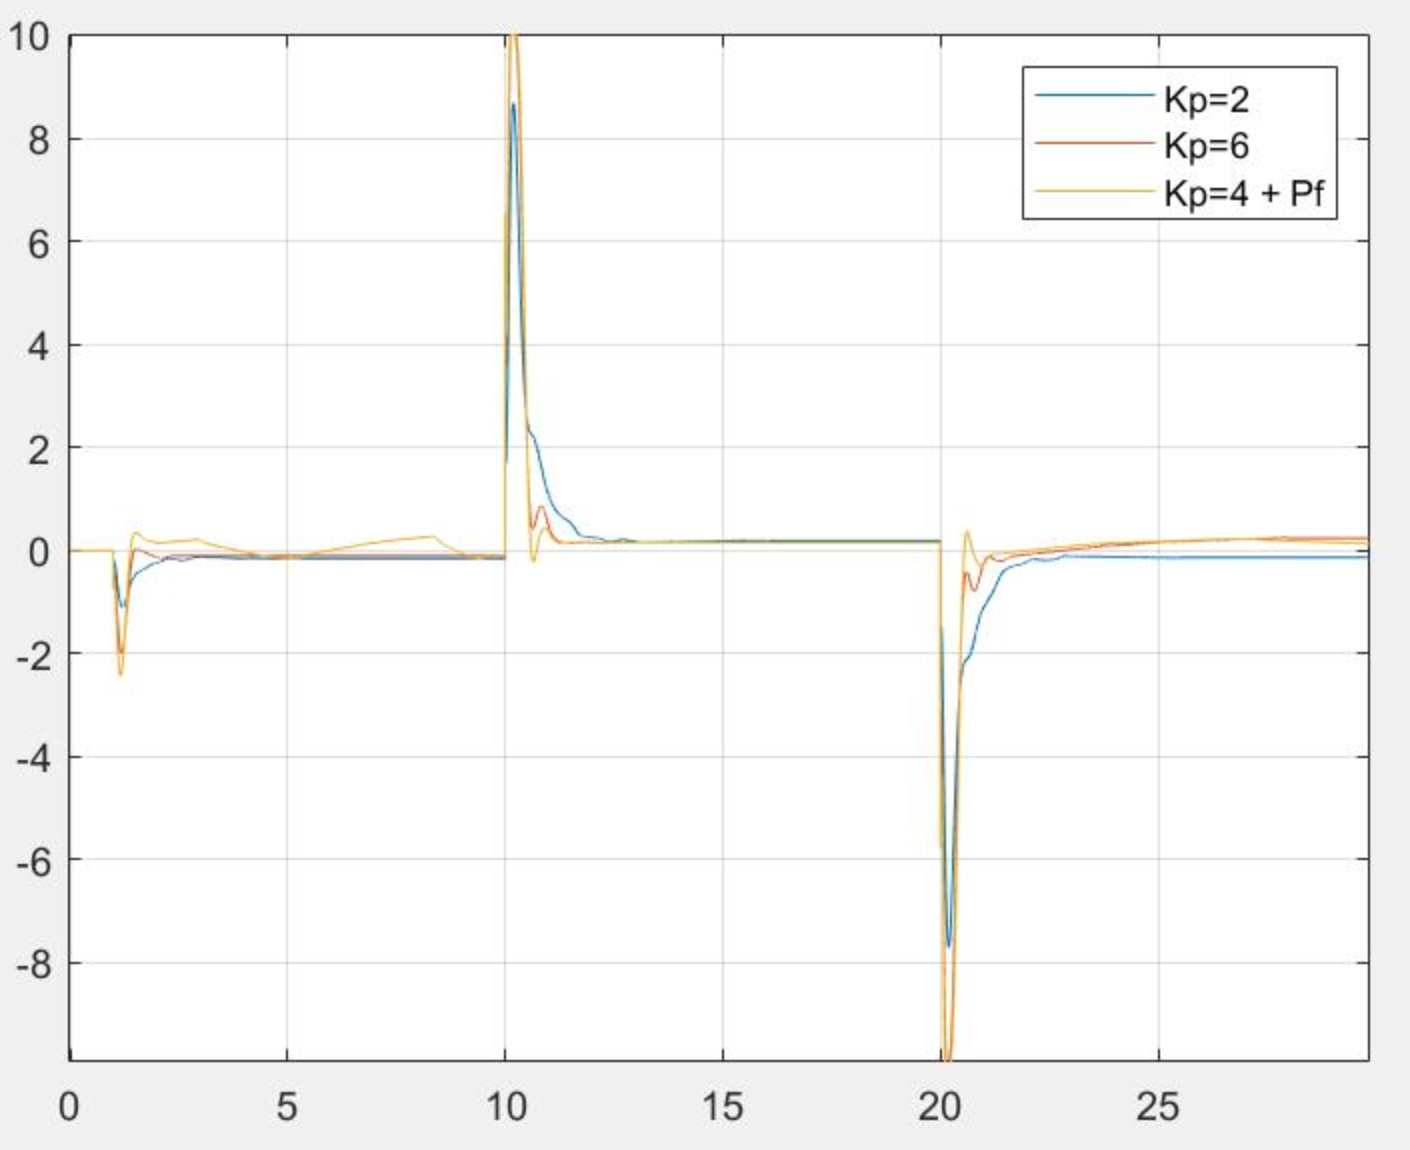
\includegraphics[scale=0.265]{immagini1/LAB_P_volt}}
	\caption{Comparison of the three possible solutions}
	\label{fig:Comparison_P_LAB}
\end{figure}

\par 
Considering the absence of overshoot and the optimal settling time we choose for the P controller made with $k_{p}$=6 rad/s.

	\chapter {2-DOF System}
We consider as transfer function from voltage to the second mass speed:

%\[	
%G(s)=
%\frac{-6.218*10^{-12}*s^4 - 1.63*10^{-10}*s^3 - 3.202*10^{-8}*s^2 - 1.413*10^{8}*s + 5.709*10^{-6}}
%{s^6 + 44.62*s^5 + 4789*s^4 + 1.831*10^{5}*s^3 + 3.262*10^{6}*s^2 + 8.035*10^{7}*s + 1.269*10^{-6}}
%\]
\begin{figure}[h]
	\centering
	\subfigure[Bode]{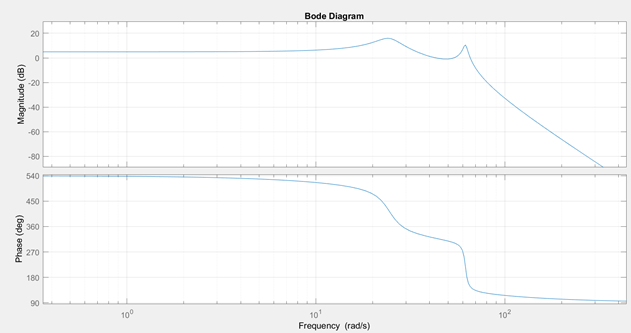
\includegraphics[scale=0.5]{immagini2/Bode_G_2_DOF}}\quad
	\subfigure[Poles and Zeros]{\includegraphics[scale=0.4]{immagini2/PZ_G}}
	\caption{G(s)}
\end{figure}

We have two uncertain resonance frequencies, by using a double notch filter, we try to attenuate the two complex poles couples respectively at 24.5 rad/s and 61.9 rad/s.
\newline
Applying the notch filter represented in figure \ref{fig:Plant G(s)with Notch Filter2}(a), we obtain the plant of figure \ref{fig:Plant G(s)with Notch Filter2}(b) that is the one we are going to control.
\begin{figure}[h]
	\centering
	\subfigure[Bode of G(s) and Nf(s)]
	{\includegraphics[scale=0.45]{immagini2/Nf_G}}\quad
	\subfigure[Bode of $G_{tot}$(s)]{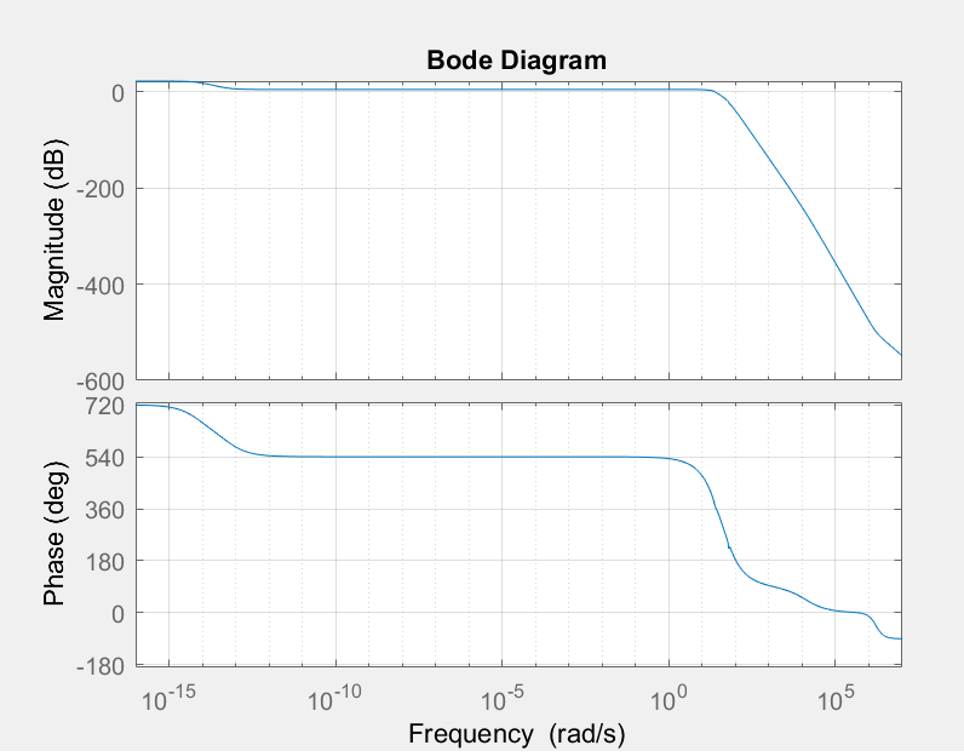
\includegraphics[scale=0.35]{immagini2/G_tot}}
	\caption{Plant G(s)with Notch Filter: $G_{tot}$(s)}
	\label{fig:Plant G(s)with Notch Filter2}
\end{figure}
\\ \\ \\ \\
\section{Speed Control Loop}
\subsection{Preliminary simulations}
We use a PI-regulator enriched with an anti-wind-up structure; we decided then to cancel out the real pole at 33.4 rad/s.
\[
R(s)=-wc_v
\frac{\frac{s}{33.4}+1}{s}
\]
As in the 1-DOF scenario, the presence of the Notch Filter postpones the cutting frequency imposed by the PI, indeed the $wc_{v}$ written in the legends below, are referred to the same parameter written in R and not to the real bandwidth of the speed-loop.
\newline We simulate now the system controlled by different PI regulators, so that we can understand the behavior that we would rather have. We test these systems with a unitary step response in figure \ref{fig:Comparison with different $wc_{v}$}.

\begin{figure}[h]
	\centering
	\includegraphics[scale=0.695]{immagini2/Step_PI_many}
	\caption{Comparison with different $wc_{v}$}
	\label{fig:Comparison with different $wc_{v}$}
\end{figure}

We decide to analyze better the three most interesting cases, that are the ones made by $wc_{v}$: 2.5 , 3 , 3.5 rad/s.
\newline  We move now to Simulink to evaluate other important aspects, like the voltage saturation.
In order to analyze both the worst case and the typical scenarios, the speed reference profile is composed by a first step from -17 rad/s to 17 rad/s and a second step of 10 rad/s. The three different reference trackings can be examinated in figure \ref{fig:Reference tracking with different $wc_{v}$} and \ref{fig:Detail of the 10 rad/s step}

\begin{figure}[h]
	\centering
	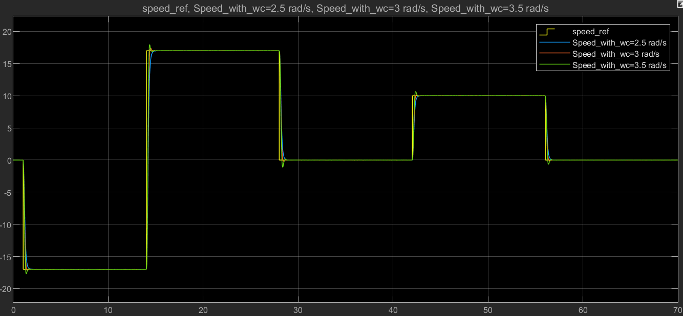
\includegraphics[scale=1.15]{immagini2/Sim_PI_Ref}
	\caption{Reference tracking with different $wc_{v}$}
	\label{fig:Reference tracking with different $wc_{v}$}
\end{figure}

\begin{figure}[h]
	\centering
	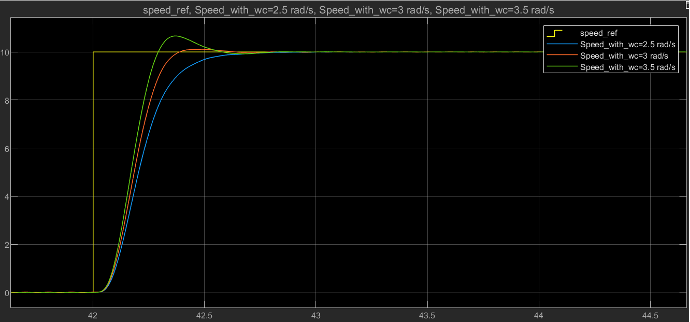
\includegraphics[scale=1.15]{immagini2/Sim_PI_10}
	\caption{Detail of the 10 rad/s step}
	\label{fig:Detail of the 10 rad/s step}
\end{figure}

We plot now the voltage signal, so as to verify whether the input action saturates or not:
\begin{itemize}
	\item $wc_{v}$ = 2.5 rad/s
	\begin{figure}[h]
		\centering
		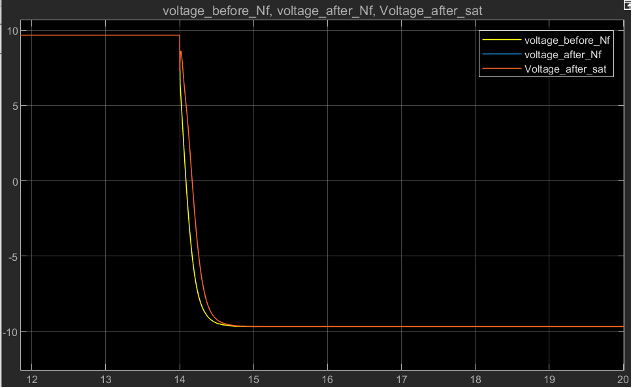
\includegraphics[scale=0.51]{immagini2/Sim_volt_2.5}
		\caption{Voltage with $wc_{v}$=2.5 rad/s}
		\label{fig:Voltage with $wc_{v}$=2.5 rad/s}
	\end{figure}
	\item $wc_{v}$ = 3 rad/s
	\begin{figure}[h]
		\centering
		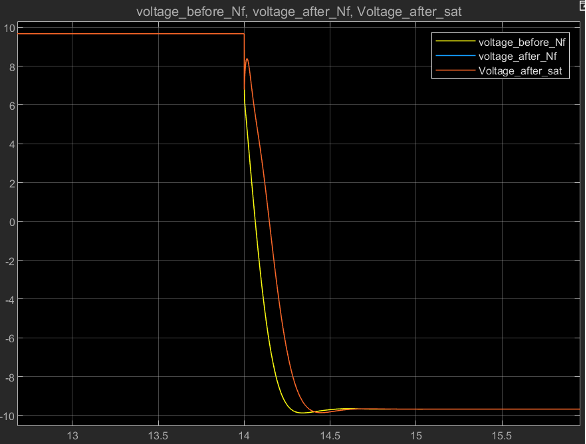
\includegraphics[scale=0.53]{immagini2/Sim_volt_3}
		\caption{Voltage with $wc_{v}$=3 rad/s}
		\label{fig:Voltage with $wc_{v}$=3 rad/s}
	\end{figure}
	\item $wc_{v}$ = 3.5 rad/s
	\begin{figure}[h]
		\centering
		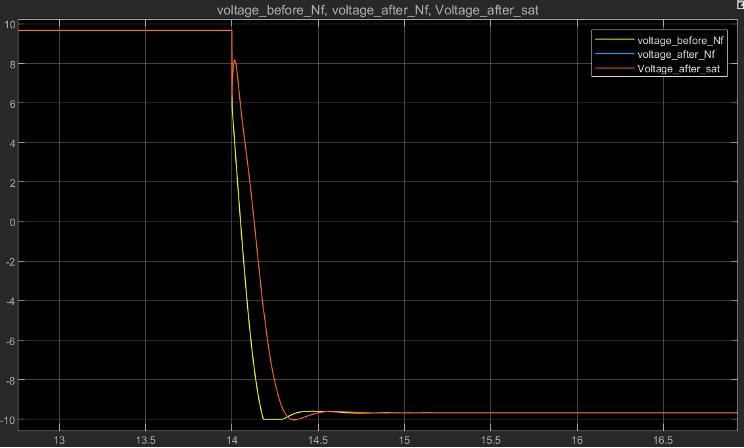
\includegraphics[scale=0.41]{immagini2/Sim_volt_3.5}
		\caption{Voltage with $wc_{v}$=3.5 rad/s}
		\label{fig:Voltage with $wc_{v}$=3.5 rad/s}
	\end{figure}
\end{itemize}

\par By analysing the previous plots, we choose $wc_{v}$= 3 rad / s that represents a good trade-off in terms of oscillations and settling time. In figure \ref{fig:Bode with $wc_{v}$=3 rad/s} we represent the bode diagram of the open loop transfer function with the above-mentioned value of $wc_{v}$.

\begin{figure}[h]
	\centering
	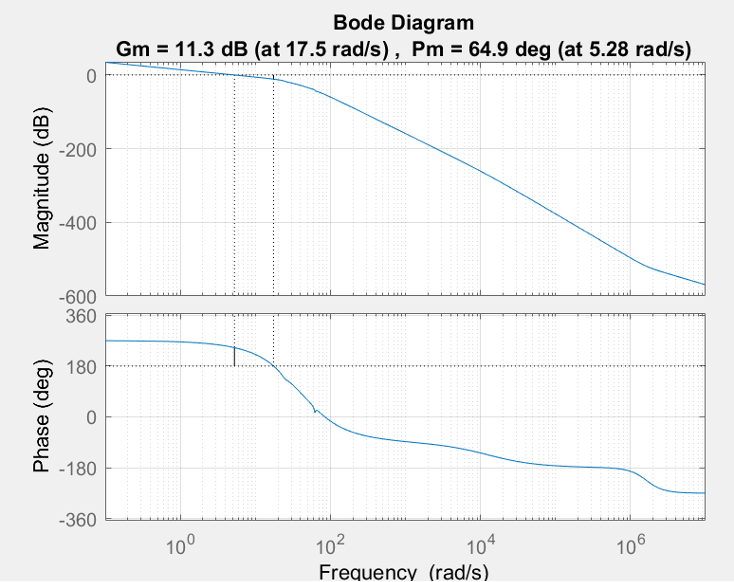
\includegraphics[scale=0.41]{immagini2/Bode_PI_3}
	\caption{Bode with $wc_{v}$=3 rad/s}
	\label{fig:Bode with $wc_{v}$=3 rad/s}
\end{figure}

\subsection{Laboratory simulations}
By doing several tests, we understand how the reasonings done at home did not take into account undesidered behavior at the steady state. Indeed, we observe the presence of very small oscillations (see figure \ref{fig:LAB_PI_5} ), their frequencies are equal to the speed, so we suppose that it depends on a change of the dynamic friction coefficient value along the revolution. As a matter of fact, this undesired behaviour can be neglected for very high speed, like 17 rad/s (because of the ratio between the amplitude of the oscillations and the reference), but they become very important for lower than 10 rad/s .  We should so increase the bandwidth of the loop to counteract them on time.  At the state of art of our control system, the goal of enlarging the bandwidth and simultaneously having a good phase margin is not feasible. To solve the problem, we need to focus on the Notch Filter. 

\begin{figure}[h]
	\centering
	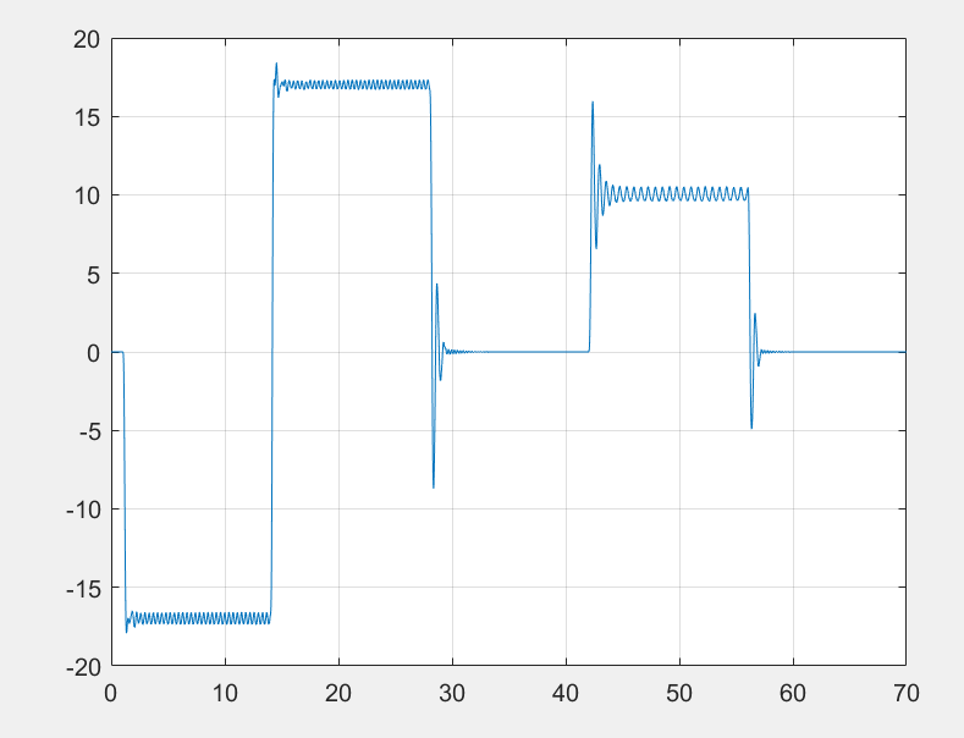
\includegraphics[scale=0.5]{immagini2/LAB_PI_5}
	\caption{Test in the laboratory with $wc_{v}$=5 rad/s}
	\label{fig:LAB_PI_5}
\end{figure}

So far, we have cancelled out the complex conjugate poles of the system and we have substituted them with higher damped poles. In this way this regulator is not too aggressive against the real dynamic of the system. As a matter of fact, to be more precise, we do not even delete the real poles of the system, but we attenuate them in a small band of 1 rad/s to be more robust against the uncertainty of the resonance peak frequencies. Anyway, to solve the problem of the above-mentioned oscillations, it is necessary to trust more on our grey box model, and to create a more aggressive regulator. In this sense, we suppose that the complex conjugate poles of the real system can be exactly cancelled, and we substitute them with other the complex conjugate poles with higher damping coefficients and resonance frequencies both at 100 rad/s (not anymore at same frequencies of the cancelled poles). Furthermore, we are allowed to enlarge the bandwidth, moving  $wc_{v}$ up to 8 rad /s. 
\newline As we can notice (see figure \ref{fig:LAB_PI_8})the oscillations at steady state are increased for 17 rad/s but they are greatly improved for 10 rad/s and they can be considered acceptable. We then decide also to test the system for low speed as 2 rad/s  since it might be one of the worst-case scenarios as regard these oscillations.

\begin{figure}[h]
	\centering
	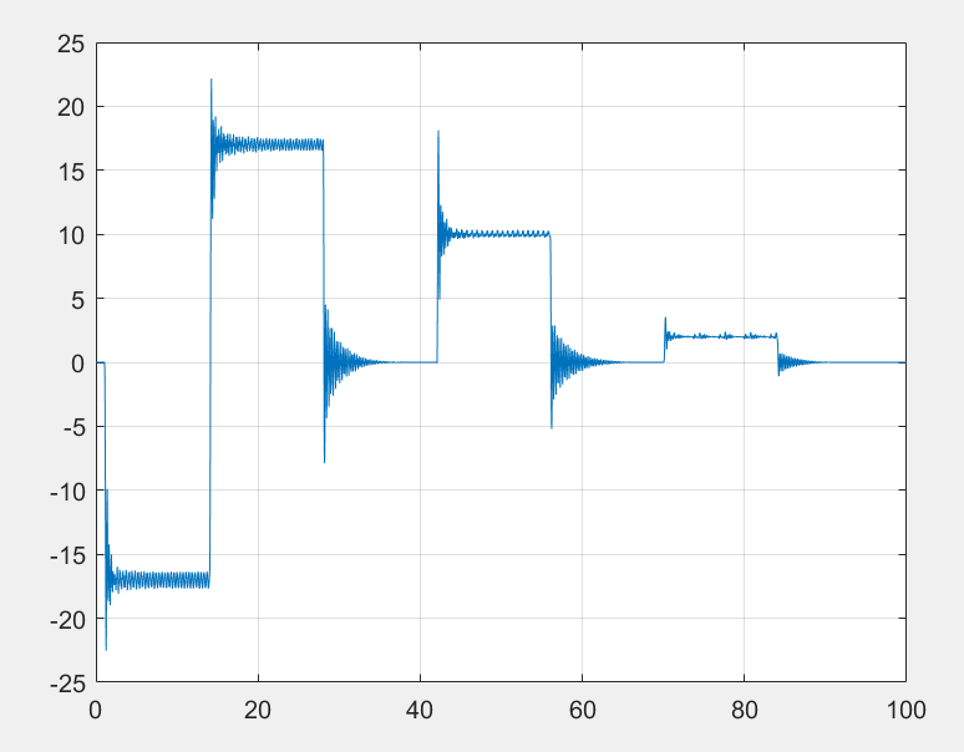
\includegraphics[scale=0.7]{immagini2/LAB_PI_8}
	\caption{Test in the laboratory with $wc_{v}$=8 rad/s and different Notch Filter}
	\label{fig:LAB_PI_8}
\end{figure}

We enlight now (see figure \ref{fig:Detail_PI})the amplitude of these oscillations for the three different reference values we applied.

\begin{figure}[h]
	\centering
	\subfigure[Reference at 17 rad/s]
	{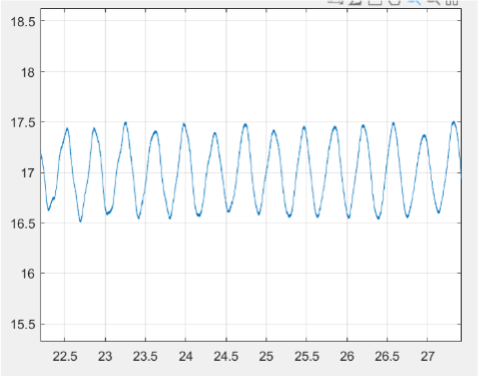
\includegraphics[scale=0.72]{immagini2/LAB_PI_17}}\quad
	\subfigure[Reference at 10 rad/s]
	{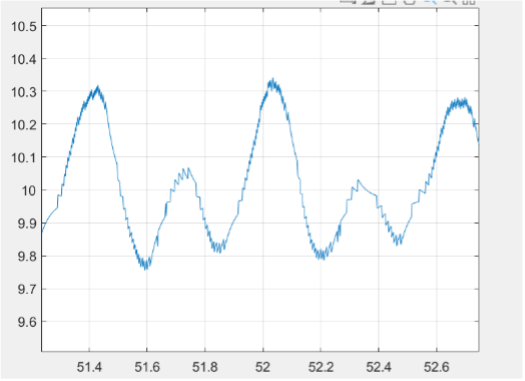
\includegraphics[scale=0.72]{immagini2/LAB_PI_10}}\quad
	\subfigure[Reference at 2 rad/s]
	{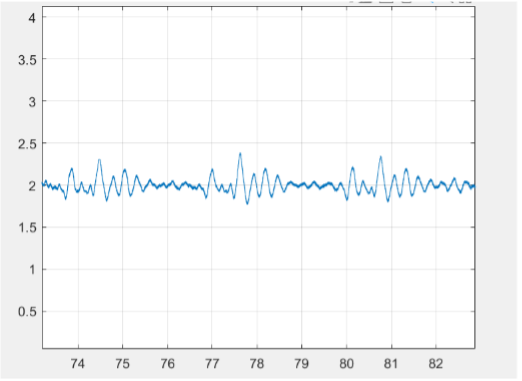
\includegraphics[scale=0.72]{immagini2/LAB_PI_2}}
	\caption{Detail of the test made with $wc_{v}$=8 rad/s }
	\label{fig:Detail_PI}
\end{figure}

The transients of this solution are far to be acceptable. Indeed, the high oscillations that we experiment in the initial instants after the steps, are related to a very low phase margin. To compensate somehow this effect, we use a low-pass pre-filter with $wc$ at 7 rad/s. Thanks to this approach, the closed loop system never receives a step as input reference, and so the control action will be smoother. As we can notice, the result is highly improved.

\begin{figure}[h]
	\centering
	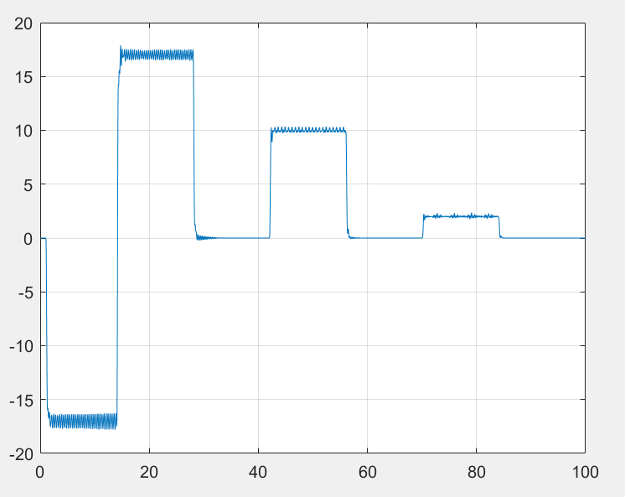
\includegraphics[scale=0.7]{immagini2/LAB_PI_Pf}
	\caption{Test made with $wc_{v}$=8 rad/s and pre-filter}
	\label{fig:LAB_PI_8}
\end{figure}

We want now to estimate the controllability range of the speed control loop. We apply so a ramp, that starts at 17 rad/s and ends to 0 rad/s.  We can observe (see figure \ref{fig:Ramp_PI}) that below 1.4 rad/s, the oscillations are so high that their amplitude might be 70/80\% of the reference. It is so not advisable to use our controller at those velocities.

\begin{figure}[h]
	\centering
	\subfigure[Entire test]
	{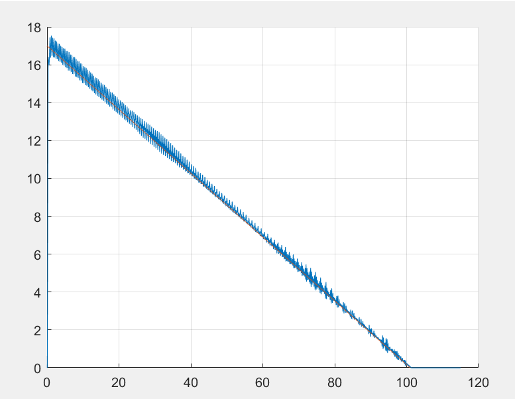
\includegraphics[scale=0.6]{immagini2/LAB_PI_RAMPa}}\quad
	\subfigure[Detail at low speed]
	{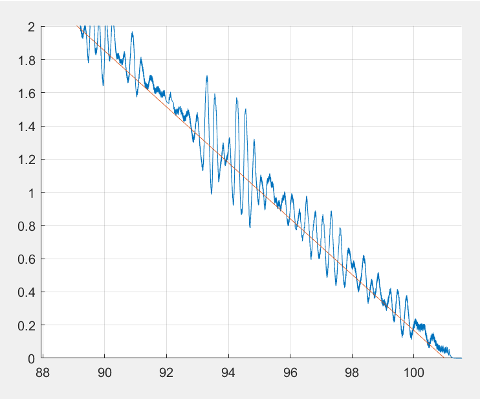
\includegraphics[scale=0.6]{immagini2/LAB_PI_RAMPb}}
	\caption{Ramp from 17 rad/s to 0 rad/s}
	\label{fig:Ramp_PI}
\end{figure}

We apply finally, a sine-sweep to verify the bandwidth of the overall system. As expected, the low pass prefilter at 7 rad/s cuts the bandwidth of closed loop system, and to prove it we can observe in the plots below (sine sweep reference from 0.1 Hz to 5 Hz in 100 seconds). Indeed, at 22s, around 7 rad/s, we can notice an attenuation of the signal around -3dB with a phase shift about 45 degrees. Due to the presence of noise and some oscillations, these values are not equal to the theoretical ones.

\begin{figure}[h]
	\centering
	\subfigure[Entire test]
	{\includegraphics[scale=0.6]{immagini2/Sine_PIa}}
	\subfigure[Detail around 7 rad/s]
	{\includegraphics[scale=0.6]{immagini2/Sine_PIb}}
	\caption{Sinesweep from 0.1 Hz  to 5 Hz}
	\label{fig:Sine_PI}
\end{figure}

\section{Position Control Loop}
\subsection{Preliminary simulations}
Following the same reasoning of the 1-DOF case, we use a cascade control strategy; it is so advisable to impose about one decade of distance between the speed and the position bandwidths. We should set a position cutting frequency about 0.5 rad/s. Since we use a proportional controller, we can simply set a gain of 0.5. However, this solution cannot be accepted since the resulting system would be too slow, as it can be seen in figure \ref{fig:Bode_P_0.5}.

\begin{figure}[h]
	\centering
	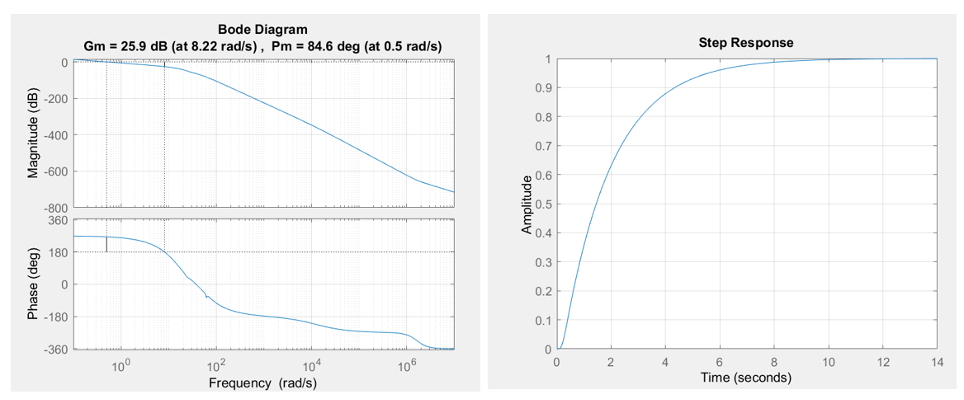
\includegraphics[scale=0.7]{immagini2/Bode_Step_P_0.5}
	\caption{Bode and step response with $k_{p}$=0.5}
	\label{fig:Bode_P_0.5}
\end{figure}

If we give less importance to the speed oscillations, we can so increase its bandwidth up to 6 rad/s (by imposing $wc_{v}$=3.5 rad/s). Now we can fix the proportional gain at 2.5. As a result, we obtain the  open loop position function plotted in the figure \ref{fig:Bode_P_2.5}.

\begin{figure}[h]
	\centering
	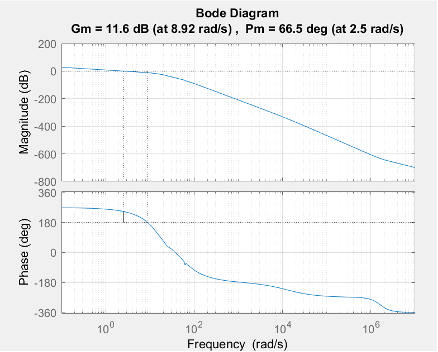
\includegraphics[scale=0.85]{immagini2/Bode_P_2.5}
	\caption{Bode  with $k_{p}$=2.5}
	\label{fig:Bode_P_2.5}
\end{figure}

On one hand, the phase margin of this solution is good and lets us have no dynamic oscillations, but on the other hand the settling time is not totally satisfying. We try so to use a high pass pre-filter on the reference signal and we compare the two solutions.
\[
P_{f}(s)=\frac{\frac{s}{2.5}+1}{\frac{s}{8}+1}
\]

\begin{figure}[h]
	\centering
	\subfigure[Tracking reference]
	{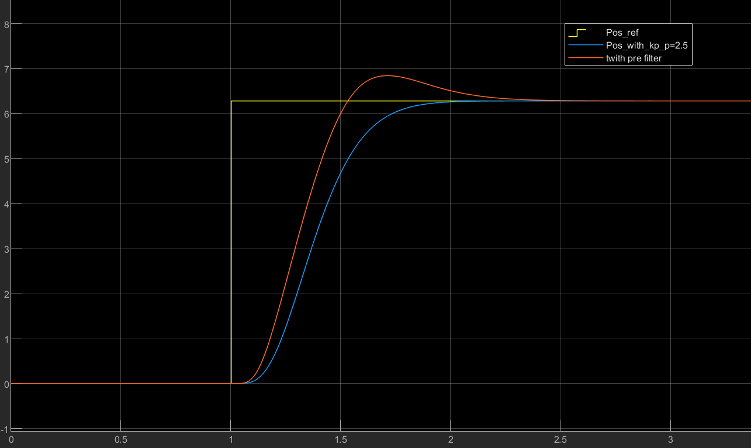
\includegraphics[scale=0.7]{immagini2/Step_P_2.5}}
	\subfigure[Voltage]
	{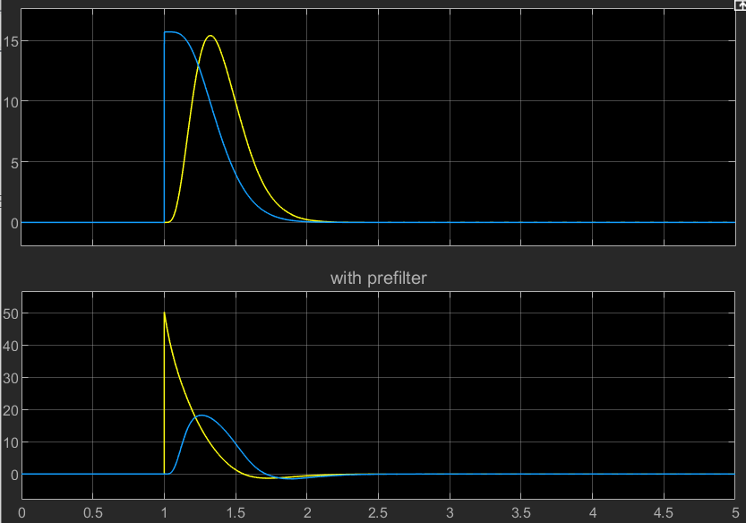
\includegraphics[scale=0.7]{immagini2/Volt_P_2.5}}
	\caption{Comparison between with and without pre-filter}
	\label{fig:Comp_P}
\end{figure}

Looking at the figure \ref{fig:Comp_P}, we would rather use the solution without the pre-filter. By the way, if the application of our system would require a faster response, the overshoot caused by the pre-filter might be considered acceptable.
\subsection{Laboratory experiments}
As discussed in the simulation part, we choose $wc_{v}$= 3.5 rad/s for the inner speed loop and now we test two values of the proportional controller for the position, $k_{p}$ equal to 2 and 2.2.
Furthermore, we then try to speed up the system with the first controller by using an high-pass prefilter $P_{f}$(s).  We would rather choose the one with $k_{p}$=2.2. 
\[
P_{f}(s)=\frac{\frac{s}{2}+1}{\frac{s}{4}+1}
\]
\\

\begin{figure}[h]
	\centering
	\includegraphics[scale=0.8]{immagini2/LAB_P_2.5}
	\caption{Reference tracking with different $k_{p}$}
\end{figure}

Due to the friction, the position reached by the two masses is not exactly the reference one. 
The controller integrates this small error and the control input raises slowly. Because the static friction coefficient is higher than the dynamic one, the load will move only after a few seconds, during which the controller has kept integrating the error asking for an increasing control action. \newline Once that the input is enough large to counteract the static friction, the load moves and the friction decreases, making the applied control input stronger than what needed. The result is that the load moves over the reference, generating an error that is even bigger than the original one.

\begin{figure}[h]
	\centering
	\includegraphics[scale=0.7]{immagini2/Static_friction}
	\caption{Detail of the position steady state error}
\end{figure}

\par For the above-mentioned reasons, we use a switch logic that deactivates the integrative action of the inner loop whenever the position error is smaller than a threshold equal to 0.85 degrees.







